\documentclass[tikz,border=5pt]{standalone}
\usepackage{tikz}
\usetikzlibrary{3d}
\usepackage{amssymb}
\usepackage{subfig}
\usepackage{float}
%\usepackage{subfigure}
\usepackage{hyperref}
\hypersetup{colorlinks=true,linkcolor=blue}
\usepackage{amsmath}
\usepackage{tikz}
\usepackage{lipsum}
\usetikzlibrary{arrows.meta}
\usetikzlibrary{arrows}
\usepackage{pstricks}
\usetikzlibrary{fadings}
%\usepackage{graphicx}
% \usepackage[nodots,nocompress]{numcompress}
\definecolor{ig}{rgb}{0.07, 0.53, 0.03}
\definecolor{cd}{rgb}{0.89, 0.0, 0.13}

\begin{document}

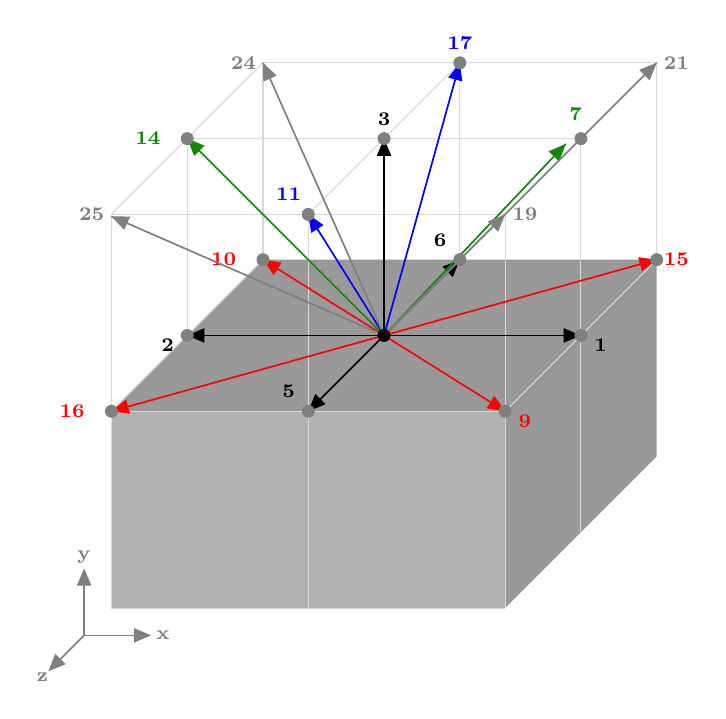
\begin{tikzpicture}[font=\scriptsize,scale=2.50,rotate around y=0,rotate around z=0]
	%	\begin{tikzpicture}[font=\scriptsize,scale=2.50,rotate around y=0,rotate around y=0]
	\tikzset{
		myarrow/.style={
				draw=#1,
				fill=#1,
				solid,
				line width=0.2mm,
				preaction={-triangle 45,#1,thin,draw,shorten <=1mm, shorten >=0mm}
			}
	}

	\fill[gray!60] (-1,-1,1) -- (1,-1,1) -- (1,0,1) -- (-1,0,1) -- cycle;
	\fill[gray!80] (1,-1,1) -- (1,0,1) -- (1,0,-1) -- (1,-1,-1) -- cycle;
	\fill[gray!80] (-1,0,1) -- (1,0,1) -- (1,0,-1) -- (-1,0,-1) -- cycle;

	\draw[solid,thin,gray!30] (-1,-1,1) -- (1,-1,1);
	\draw[solid,thin,gray!30] (-1,0,1) -- (1,0,1);

	\draw[solid,thin,gray!30] (-1,-1,1) -- (-1,0,1);
	\draw[solid,thin,gray!30] (1,-1,1) -- (1,0,1);
	\draw[solid,thin,gray!30] (0,-1,1) -- (0,0,1);

	\draw[solid,thin,gray!30] (-1,0,1) -- (-1,0,-1);
	\draw[solid,thin,gray!30] (1,0,1) -- (1,0,-1);
	\draw[solid,thin,gray!30] (0,0,1) -- (0,0,-1);

	\draw[solid,thin,gray!30] (-1,0,0) -- (1,0,0);
	\draw[solid,thin,gray!30] (1,-1,0) -- (1,0,0);

	%upper part

	\draw[solid,thin,gray!30] (-1,0,0) -- (1,0,0);

	\draw[thin,gray!30] (-1,0, 1) -- (1,0, 1) -- (1,1, 1) -- (-1,1, 1) -- cycle;
	\draw[thin,gray!30] (-1,0, -1) -- (1,0, -1) -- (1,1, -1) -- (-1,1, -1) -- cycle;
	\draw[thin,gray!30] (-1,0, 0) -- (1,0, 0) -- (1,1, 0) -- (-1,1, 0) -- cycle;

	\draw[solid,thin,gray!30] (-1,1,1) -- (-1,1,-1);
	\draw[solid,thin,gray!30] (0,1,1) -- (0,1,-1);
	\draw[solid,thin,gray!30] (1,1,1) -- (1,1,-1);

	\draw[solid,thin,gray!30] (0,0,1) -- (0,1,1);
	\draw[solid,thin,gray!30] (0,0,-1) -- (0,1,-1);

	\draw[solid,thin,gray!30] (0,0,0) -- (0,1,0);

	% Node 1
	\path[myarrow=black, fill=red] (0,0,0) -- (1,0,0);
	\draw (1.1,-0.05,0) node {$\mathbf{1}$};

	% Node 2
	\path[myarrow=black, fill=black] (0,0,0) -- (-1,0,0);
	\draw (-1.1,-0.05,0) node {$\mathbf{2}$};

	% Node 3
	\path[myarrow=black, fill=black] (0,0,0) -- (0,1,0);
	\draw (0,1.1,0) node {$\mathbf{3}$};

	% Node 5
	\path[myarrow=black, fill=black] (0,0,0) -- (0,0,1);
	\draw (-0.1,0.1,1) node {$\mathbf{5}$};

	% Node 6
	\path[myarrow=black, fill=black] (0,0,0) -- (0,0,-1);
	\draw (-0.1,0.1,-1) node {$\mathbf{6}$};

	% Node 7
	\path[myarrow=ig] (0,0,0) -- (1,1.05,0.2);
	\draw (1.05,1.2,0.2) node[ig] {$\mathbf{7}$};

	% Node 14
	\path[myarrow=ig] (0,0,0) -- (-1,1,0);
	\draw (-1.2,1,0) node[ig] {$\mathbf{14}$};

	% Node 9
	\path[myarrow=red] (0,0,0) -- (1,0,1);
	\draw (1.1,-0.05,1) node[red] {$\mathbf{9}$};

	% Node 10
	\path[myarrow=red] (0,0,0) -- (-1,0,-1);
	\draw (-1.2,0,-1) node[red] {$\mathbf{10}$};

	% Node 15
	\path[myarrow=red] (0,0,0) -- (1,0,-1);
	\draw (1.1,0,-1) node[red] {$\mathbf{15}$};

	% Node 16
	\path[myarrow=red] (0,0,0) -- (-1,0,1);
	\draw (-1.2,0,1) node[red] {$\mathbf{16}$};

	% Node 11
	\path[myarrow=blue] (0,0,0) -- (0,1,1);
	\draw (-0.1,1.1,1) node[blue] {$\mathbf{11}$};

	% Node 17
	\path[myarrow=blue] (0,0,0) -- (0,1,-1);
	\draw (0,1.1,-1) node[blue] {$\mathbf{17}$};

	% Node 19
	%\draw[gray,fill=gray] (1,1,1)node[]{} circle(0.03cm);  %node 19
	\path[myarrow=gray] (0,0,0) -- (1,1,1);
	\draw (1.1,1,1) node[gray] {$\mathbf{19}$};
	\\
	% Node 21
	%\draw[gray,fill=gray] (1,1,-1)node[]{} circle(0.03cm);  %node 21
	\path[myarrow=gray] (0,0,0) -- (1,1,-1);
	\draw (1.1,1,-1) node[gray] {$\mathbf{21}$};

	% Node 24
	%\draw[gray,fill=gray] (-1,1,-1)node[]{} circle(0.03cm);  %node 24
	\path[myarrow=gray] (0,0,0) -- (-1,1,-1);
	\draw (-1.1,1,-1) node[gray] {$\mathbf{24}$};

	% Node 25
	%\draw[gray,fill=gray] (-1,1,1)node[]{} circle(0.03cm);  %node 25
	\path[myarrow=gray] (0,0,0) -- (-1,0.99,1);
	\draw (-1.1,1,1) node[gray] {$\mathbf{25}$};

	\draw[black,fill=black] (0,0,0)node[]{} circle(0.03cm); %node 0
	\draw[gray,fill=gray] (1,0,0)node[]{} circle(0.03cm);  %node 1
	\draw[gray,fill=gray] (-1,0,0)node[]{} circle(0.03cm);  %node 2
	\draw[gray,fill=gray] (0,1,0)node[]{} circle(0.03cm);  %node 3
	\draw[gray,fill=gray] (0,0,1)node[]{} circle(0.03cm);  %node 5
	\draw[gray,fill=gray] (0,0,-1)node[]{} circle(0.03cm);  %node 6
	\draw[gray,fill=gray] (1,1,0)node[]{} circle(0.03cm);  %node 7
	\draw[gray,fill=gray] (1,0,1)node[]{} circle(0.03cm);  %node 9
	\draw[gray,fill=gray] (-1,0,-1)node[]{} circle(0.03cm);  %node 10
	\draw[gray,fill=gray] (0,1,1)node[]{} circle(0.03cm);  %node 11
	\draw[gray,fill=gray] (-1,1,0)node[]{} circle(0.03cm);  %node 14
	\draw[gray,fill=gray] (1,0,-1)node[]{} circle(0.03cm);  %node 15
	\draw[gray,fill=gray] (-1,0,1)node[]{} circle(0.03cm);  %node 16
	\draw[gray,fill=gray] (0,1,-1)node[]{} circle(0.03cm);  %node 17

	\path[draw=gray,solid,line width=0.2mm,preaction={-triangle 45,gray,thin,draw,shorten >=-1mm}](-1.1,-1.1,1.1) -- (-0.8,-1.1,1.1);	%node x
	\draw (-0.7,-1.1,1.1)node[gray]{$\mathbf{x}$};
	\path[draw=gray,solid,line width=0.2mm,preaction={-triangle 45,gray,thin,draw,shorten >=-1mm}](-1.1,-1.1,1.1) -- (-1.1,-0.8,1.1);	%node y
	\draw (-1.1,-0.7,1.1)node[gray]{$\mathbf{y}$};
	\path[draw=gray,solid,line width=0.2mm,preaction={-triangle 45,gray,thin,draw,shorten >=-1mm}](-1.1,-1.1,1.1) -- (-1.1,-1.1,1.5);	%node z
	\draw (-1.1,-1.1,1.65)node[gray]{$\mathbf{z}$};
\end{tikzpicture}

\end{document}
